\documentclass[12pt, a4paper]{article}
\usepackage{amsmath}
\usepackage{amssymb}
\usepackage[style=authoryear, backend=biber, maxnames=3]{biblatex} % for the citation, 
\usepackage{hyperref}
\addbibresource{bibentries.bib}

\usepackage{graphicx}
\usepackage[utf8]{inputenc}
\setlength\parindent{0pt}

\title{Here goes the title}
\author{ABC\thanks{ABC Universität}\ , 
CDE\thanks{CDE Universität} \ and 
David Zimmermann\footnotemark[2]\
 \thanks{Correspondence should be addressed to David Zimmermann, Zeppelin Universität, Am Seemooser Horn 20 in D-88045 Friedrichshafen, Germany. E-mail: david.zimmermann@zu.de}}
\date{Working Paper version \today}

\begin{document}
\maketitle

\rule{\linewidth}{0.4pt}
\begin{abstract}
This is the abstract
\end{abstract}
\textbf{Keywords:} asdasd, asd, asd\\
\medskip
\textbf{JEL codes:} asdasd, asd, asd\\
\rule{\linewidth}{0.4pt}

\section{Introduction}
This work cites \textcite{Brealey2012}, but also \textcite{Modigliani1958}. 


\begin{figure}
\caption{A Figure using R}
\centering
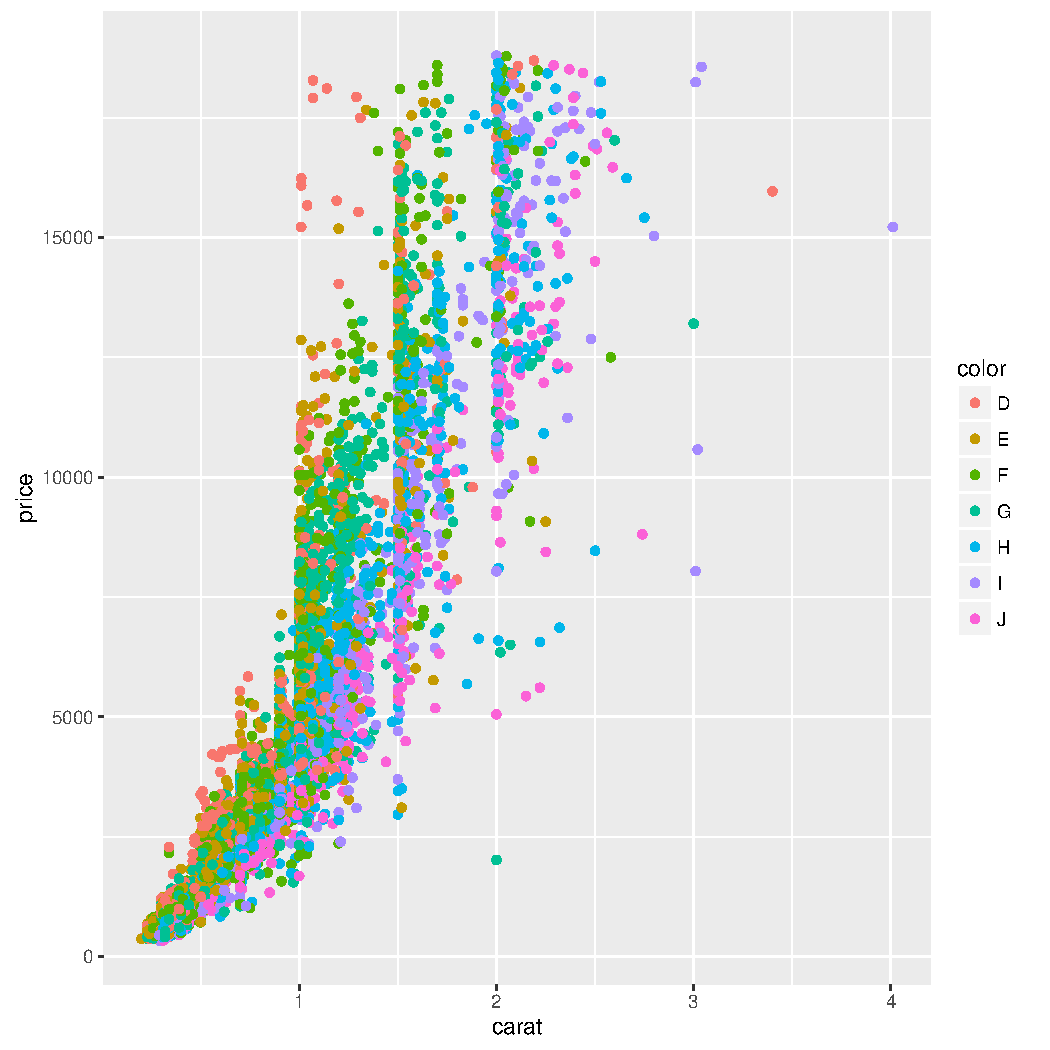
\includegraphics[width=0.75\textwidth]{figures/fig1}
\end{figure}

\begin{table}
\begin{scriptsize}

% Table created by stargazer v.5.2 by Marek Hlavac, Harvard University. E-mail: hlavac at fas.harvard.edu
% Date and time: Do, Aug 25, 2016 - 21:13:05
\begin{tabular}{@{\extracolsep{5pt}}lccc} 
\\[-1.8ex]\hline 
\hline \\[-1.8ex] 
 & \multicolumn{3}{c}{\textit{Dependent variable:}} \\ 
\cline{2-4} 
\\[-1.8ex] & \multicolumn{3}{c}{price} \\ 
\\[-1.8ex] & (1) & (2) & (3)\\ 
\hline \\[-1.8ex] 
 carat & 8,011.947$^{***}$ & 10,777.200$^{***}$ & 7,705.113$^{***}$ \\ 
  & (32.120) & (133.902) & (32.429) \\ 
  & & & \\ 
 colorE & $-$170.950$^{***}$ & $-$167.414$^{***}$ &  \\ 
  & (53.190) & (51.554) &  \\ 
  & & & \\ 
 colorF & $-$129.433$^{**}$ & $-$113.864$^{**}$ &  \\ 
  & (53.284) & (51.671) &  \\ 
  & & & \\ 
 colorG & $-$78.364 & $-$63.592 &  \\ 
  & (51.969) & (50.375) &  \\ 
  & & & \\ 
 colorH & $-$725.887$^{***}$ & $-$730.633$^{***}$ &  \\ 
  & (55.561) & (53.863) &  \\ 
  & & & \\ 
 colorI & $-$1,053.623$^{***}$ & $-$1,134.314$^{***}$ &  \\ 
  & (62.623) & (60.751) &  \\ 
  & & & \\ 
 colorJ & $-$1,992.605$^{***}$ & $-$2,061.031$^{***}$ &  \\ 
  & (77.448) & (75.105) &  \\ 
  & & & \\ 
 depth & $-$96.938$^{***}$ &  &  \\ 
  & (10.045) &  &  \\ 
  & & & \\ 
 x &  & $-$4,378.231$^{***}$ &  \\ 
  &  & (267.559) &  \\ 
  & & & \\ 
 y &  & 4,224.406$^{***}$ &  \\ 
  &  & (264.373) &  \\ 
  & & & \\ 
 z &  & $-$1,680.926$^{***}$ &  \\ 
  &  & (136.679) &  \\ 
  & & & \\ 
 vol & $-$0.078$^{***}$ & 0.348$^{***}$ & $-$0.098$^{***}$ \\ 
  & (0.013) & (0.029) & (0.014) \\ 
  & & & \\ 
 Constant & 3,902.612$^{***}$ & 2,481.167$^{***}$ & $-$2,226.144$^{***}$ \\ 
  & (620.807) & (229.725) & (30.124) \\ 
  & & & \\ 
\hline \\[-1.8ex] 
Observations & 10,000 & 10,000 & 10,000 \\ 
R$^{2}$ & 0.867 & 0.875 & 0.850 \\ 
Adjusted R$^{2}$ & 0.866 & 0.874 & 0.850 \\ 
Residual Std. Error & 1,447.821 (df = 9990) & 1,403.304 (df = 9988) & 1,533.963 (df = 9997) \\ 
F Statistic & 7,205.859$^{***}$ (df = 9; 9990) & 6,334.414$^{***}$ (df = 11; 9988) & 28,337.980$^{***}$ (df = 2; 9997) \\ 
\hline 
\hline \\[-1.8ex] 
\textit{Note:}  & \multicolumn{3}{r}{$^{*}$p$<$0.1; $^{**}$p$<$0.05; $^{***}$p$<$0.01} \\ 
\end{tabular} 

\end{scriptsize}
\caption{A table using stargazer}
\end{table}

\begin{table}
\begin{scriptsize}

% Table created by stargazer v.5.2 by Marek Hlavac, Harvard University. E-mail: hlavac at fas.harvard.edu
% Date and time: Do, Aug 25, 2016 - 21:13:06
\begin{tabular}{@{\extracolsep{5pt}}lcc} 
\\[-1.8ex]\hline 
\hline \\[-1.8ex] 
 & \multicolumn{2}{c}{\textit{Dependent variable:}} \\ 
\cline{2-3} 
\\[-1.8ex] & \multicolumn{2}{c}{price} \\ 
\\[-1.8ex] & (1) & (2)\\ 
\hline \\[-1.8ex] 
 carat & 8,011.947$^{***}$ & 10,777.200$^{***}$ \\ 
  & (32.120) & (133.902) \\ 
  & & \\ 
 colorE & $-$170.950$^{***}$ & $-$167.414$^{***}$ \\ 
  & (53.190) & (51.554) \\ 
  & & \\ 
 colorF & $-$129.433$^{**}$ & $-$113.864$^{**}$ \\ 
  & (53.284) & (51.671) \\ 
  & & \\ 
 colorG & $-$78.364 & $-$63.592 \\ 
  & (51.969) & (50.375) \\ 
  & & \\ 
 colorH & $-$725.887$^{***}$ & $-$730.633$^{***}$ \\ 
  & (55.561) & (53.863) \\ 
  & & \\ 
 colorI & $-$1,053.623$^{***}$ & $-$1,134.314$^{***}$ \\ 
  & (62.623) & (60.751) \\ 
  & & \\ 
 colorJ & $-$1,992.605$^{***}$ & $-$2,061.031$^{***}$ \\ 
  & (77.448) & (75.105) \\ 
  & & \\ 
 depth & $-$96.938$^{***}$ &  \\ 
  & (10.045) &  \\ 
  & & \\ 
 x &  & $-$4,378.231$^{***}$ \\ 
  &  & (267.559) \\ 
  & & \\ 
 y &  & 4,224.406$^{***}$ \\ 
  &  & (264.373) \\ 
  & & \\ 
 z &  & $-$1,680.926$^{***}$ \\ 
  &  & (136.679) \\ 
  & & \\ 
 vol & $-$0.078$^{***}$ & 0.348$^{***}$ \\ 
  & (0.013) & (0.029) \\ 
  & & \\ 
 Constant & 3,902.612$^{***}$ & 2,481.167$^{***}$ \\ 
  & (620.807) & (229.725) \\ 
  & & \\ 
\hline \\[-1.8ex] 
Observations & 10,000 & 10,000 \\ 
R$^{2}$ & 0.867 & 0.875 \\ 
Adjusted R$^{2}$ & 0.866 & 0.874 \\ 
Residual Std. Error & 1,447.821 (df = 9990) & 1,403.304 (df = 9988) \\ 
F Statistic & 7,205.859$^{***}$ (df = 9; 9990) & 6,334.414$^{***}$ (df = 11; 9988) \\ 
\hline 
\hline \\[-1.8ex] 
\textit{Note:}  & \multicolumn{2}{r}{$^{*}$p$<$0.1; $^{**}$p$<$0.05; $^{***}$p$<$0.01} \\ 
\end{tabular} 

\end{scriptsize}
\caption{Another table using stargazer}
\end{table}

\newpage

\printbibliography
\end{document}